后端业务、算法、权限及交付校验180项通过，浏览器师生流程与交互回归共34项通过。界面检查覆盖两门课程的师生19个业务模块及登录入口，采用四种桌面视口与手机窄屏，共保存480张截图。常规回归使用本地示例模式。真实模型验证共202次请求，官方用量为297521输入和73783输出Token；另以保守预留计入未知消耗，累计控制额为371304Token。

\subsection{实验对象、划分与评价}
实验固定随机种子101711，沿用正式服务的知识更新、路径搜索、分组与检索函数。开发集用于检查生成器、返回格式和评分程序，评测集在任务执行前固定。知识轨迹按学生序列划分，路径按独立图划分，检索按知识主题划分，同一主题的改写进入同一分区。输入和逐例输出均保留，失败计入对应分母。
\begin{table}[htbp]\centering\caption{本地实验的独立对象与场景}\begin{tabularx}{\linewidth}{Yrrr}\toprule 实验&开发&评测&场景说明\\\midrule 知识追踪&120条&1200条&25920次学习事件\\路径规划&20图&180图&每图4预算，共720例\\教学分层&6班&48班&16—80人，共2064人\\资料检索&20问&180问&50主题、3课程\\\bottomrule\end{tabularx}\end{table}
评价依方法职责组织。轨迹误差反映合成状态下的估计差异，路径检查执行约束与效用，分层核对错因关系及任务匹配，检索核对参考来源排名与定位。真实模型另以相同任务、模型和资料进行配对，接口完成、结构合法和业务完成分别统计。所有数据为自编课程内容与合成教学记录，这些结果衡量方法机制与系统执行表现。本项目按各方法实际承担的教学职责选择指标，使计算结果能够对应到课程活动的可执行性、判断依据和教师操作。

\subsection{知识追踪的长短轨迹与消融}
轨迹长度为4、8、16、32、48，生成器以逻辑函数模拟难度、猜测、失误和提示影响，并加入随机进步、长间隔、状态突变、无遗忘及相关重复条件。潜在状态采用随机演化，作答生成与Beta更新采用不同公式。每条轨迹计算估计与潜在状态的均方根误差，再按1200条序列取平均。
\begin{figure}[htbp]\centering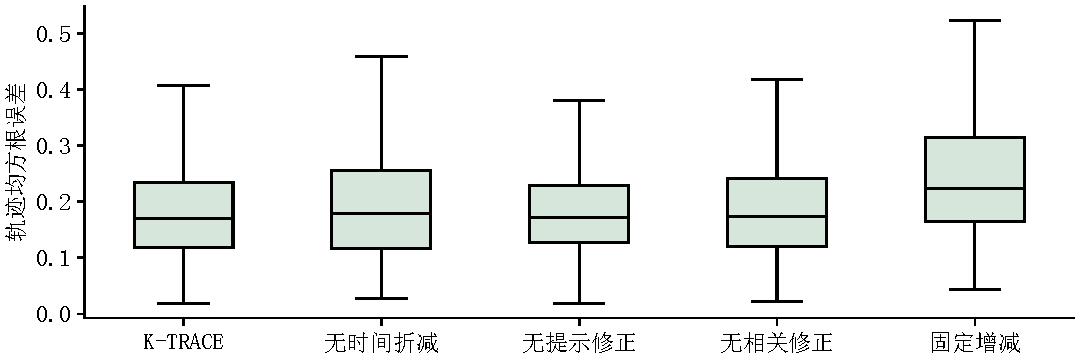
\includegraphics[width=\linewidth]{../figures/round10/ktrace-distribution.pdf}\caption{相同轨迹下的知识估计误差分布，中位数与四分位区间}\end{figure}
\begin{table}[htbp]\centering\caption{知识追踪消融的平均轨迹误差}\begin{tabularx}{\linewidth}{Yrrrrr}\toprule 方法&K-TRACE&无时间折减&无提示修正&无相关修正&固定增减\\\midrule 均方根误差&0.1865&0.1963&0.1862&0.1897&0.2437\\\bottomrule\end{tabularx}\end{table}
时间与相关性修正使长间隔和密集变式的影响分别进入计算。提示修正的整体误差与消融接近，其作用随生成条件变化；无遗忘情景中，移除时间折减的结果更好。这说明参数与课程测量条件存在联系，实际使用时可结合课程题目进一步标定。短期重复成功的零权重检查全部满足，重复作答保留学习历史，同时限制重复证据的增幅。本项目重视这种对证据来源的区分，它使同样的正确率能够表达不同的学习过程，为后续复习和教师判断提供更细致的依据。

\subsection{路径规划的可行对照与精确参考}
先修图包含6—32节点、三种关系密度、资源缺失、不同目标数以及任务与复习竞争，每图分别测试10、20、30、60分钟。可行贪心与PATH-G使用相同候选、效用、预算和先修条件，贪心逐步选择边际效用密度最高的合法活动。静态目标排序作为顺序约束的参照。小图以子集动态规划求精确参考。
\begin{figure}[htbp]\centering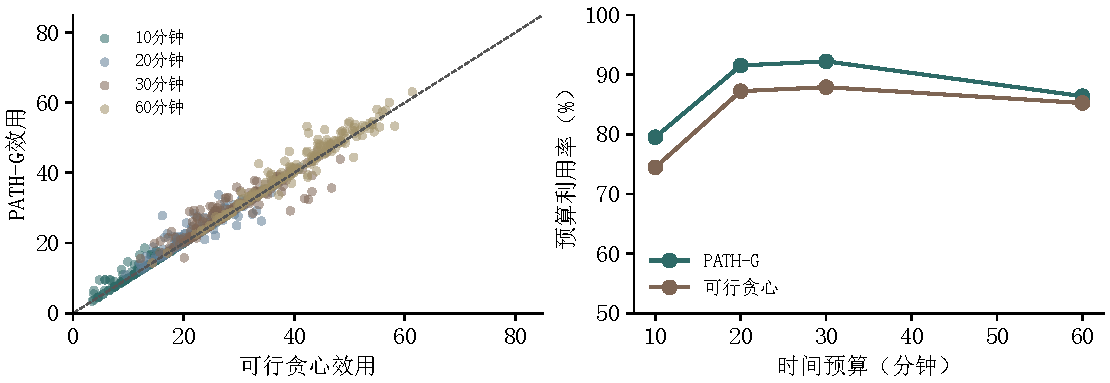
\includegraphics[width=\linewidth]{../figures/round10/path-comparison.pdf}\caption{720种场景的配对效用与预算利用率；虚线表示两方法效用相同}\end{figure}
PATH-G与可行贪心均为0次先修违规、0次预算违规。平均效用分别为27.27与26.53，相对变化2.80\%，按180个独立图聚类重采样\cite{bootstrap}的95\%区间为[2.15\%,3.48\%]。逐例比较为456胜、209平、55负，有限束搜索在部分图中保留的前缀仍可能不及贪心。288个小图预算场景中，平均达到精确参考效用的99.95\%。
预算利用率为87.41\%与83.70\%，目标覆盖率为46.02\%与43.10\%。静态目标排序覆盖率较高，但产生1477条未满足先修的依赖，因此可行对照更接近实际学习安排。PATH-G平均单次计算1.12毫秒，逐例保留搜索扩展数与更新状态后的重规划。本项目选择有限束搜索，是为了让相互依赖的活动有机会共同进入计划。更高的预算利用率与目标覆盖率说明这一设计能够在相同约束下组织更多有用活动，学生完成后的新证据再决定下一次安排。

\subsection{班级分层与检索覆盖}
48个班级共2064名合成学生，包含噪声、缺失维度、稀疏记录、混合困难和状态变化。32个明确单一错因原型班级中，CLASS-LOOP的成对关系一致率为1.0000，移除支持度为0.9860，按总困难程度四分位分组为0.6525。48班的输入重排结果均一致，稀疏记录均按观察组规则处理，184项任务推荐全部匹配群组主要薄弱知识，平均计算5.61毫秒。另设8个证据变化场景，重新分组后8/8教学关注随困难改变。支持度使未观测维度与已观测困难各自发挥作用，教师据此获得更具体的练习对象。分组与题目匹配一起执行，使分析结果能够直接成为面向当前困难的教学行动。
资料检索采用课程已有讲义与普通上传的私有附件，并通过正常接口建立信息素养单元。180问包含直接提问、无显式知识点、边界比较及附件联合检索。词项基线Top-1为176/180，知识增强和当前完整方案均为178/180；Top-5分别为179/180与180/180。完整方案与知识增强在该集合上相同，顺序术语的专门作用由比较与否定回归检验。所有返回来源均具有定位和版本，三个课程的师生私有可见性6/6正确，证据不足例返回空集。参考材料更容易进入回答上下文，师生也能够打开相应位置核对解释。

\subsection{真实模型的配对任务}
先以12次请求检查采集和计费，再执行80个独立任务，每任务两种条件，共160个正式响应。学生与教师各40任务，分别覆盖八类需求。双方共享课程资料、统计、候选对象、输出结构与长度，保留同一权限和业务校验，简化基线改为单步生成措辞。Flash承担主体，Pro用于16个正式响应。该对照考察共享业务工具条件下提示编排的增量。
\begin{table}[htbp]\centering\caption{同条件模型任务评价，分母均为80}\begin{tabularx}{\linewidth}{Yrr}\toprule 指标&原编排&单步提示\\\midrule API完成&79/80&80/80\\结构合法&77/80&80/80\\业务完成&77/80&80/80\\引用编号有效&58/80&55/80\\\bottomrule\end{tabularx}\end{table}
业务完成要求回答落库、学生有效理解检查或教师有效产物，教学设计与干预还需保存为教案。讨论和分析按其任务类型核查。引用编号的检查只判断来源编号存在，实际来源与返回原文一并保存。分类型结果和失败响应能够进一步区分接口完成与教学结果。相同证据和校验使两种提示都具备执行基础，结果差异反映具体任务的结构遵循情况。本项目据此将改进重点放在产物识别和保存环节，使已有内容更可靠地进入业务，而保留首次配对结果作为公平比较。

\subsection{输入链路、任务回流与故障复核}
20个独立业务场景覆盖TXT、Markdown、DOCX、PDF、图片理解、模型切换、教案、出题、量规与理解反馈，初次完成18/20。两例教学方案分别使用换行标记和JSON代码块，合法内容未进入保存。兼容解析后，两份原响应通过原业务校验并保存，另以8个新主题真实任务独立复核，8/8形成有效方案并保存。原始失败继续保留，修复结果分别统计。
教学场景实际创建任务，学生完成全部关联题目，教师结果页读取完成状态和得分。语音补充场景实际执行本地Whisper转写，再分别进入Flash与Pro课程问答，两个模型的记录分别保存。服务校验课程、题目、群组和课时，教师确认后进入保存与发布，学生作答再形成新的证据。
真实请求共202次，官方输入297521、输出73783 Token，保守计入控制额371304，总预算1,000,000。试运行、正式配对、业务、独立复核及输入链路分别记录。输入缓存计入总量，推理明细保留于输出统计，缺少官方用量的情况保留预留额。材料图表和结论均从已经完成的结果文件生成。
